% This is samplepaper.tex, a sample chapter demonstrating the
% LLNCS macro package for Springer Computer Science proceedings;
% Version 2.20 of 2017/10/04
%
\documentclass[runningheads]{llncs}
%
\usepackage{graphicx}
% Used for displaying a sample figure. If possible, figure files should
% be included in EPS format.
%
% If you use the hyperref package, please uncomment the following line
% to display URLs in blue roman font according to Springer's eBook style:
% \renewcommand\UrlFont{\color{blue}\rmfamily}
\usepackage{hyperref}
\newcommand{\quotes}[1]{``#1''}
\usepackage{float}
\usepackage{csvsimple}
\usepackage[T1]{fontenc}
\usepackage{tabularx}
\usepackage{siunitx}
\usepackage{rotating}
\begin{document}
%
\title{Counting Pedestrians via Webcams\thanks{Supported by organization x.}}
%
%\titlerunning{Abbreviated paper title}
% If the paper title is too long for the running head, you can set
% an abbreviated paper title here
%
\author{Yafei Yan\inst{}\orcidID{} \and
Ruikun Li\inst{}\orcidID{}}
%\and Third Author\inst{3}\orcidID{2222--3333-4444-5555}}
%
% \authorrunning{F. Author et al.}
% First names are abbreviated in the running head.
% If there are more than two authors, 'et al.' is used.
%
\institute{RWTH Aachen University, Ahornstrasse 55, 52074 Aachen, Germany 
\url{http://cssh.rwth-aachen.de/}}
% \email{lncs@springer.com}\\
% \url{http://www.springer.com/gp/computer-science/lncs} \and
% ABC Institute, Rupert-Karls-University Heidelberg, Heidelberg, Germany\\
% \email{\{abc,lncs\}@uni-heidelberg.de}}
%
\maketitle              % typeset the header of the contribution
%
\begin{abstract}
Object detection is an challenged task since machine cannot observe objects like human who can instantly recognize an object. Based on the technique of convolutional neural network (CNN) the object detection became easy. By applying the object detection here we focus on counting pedestrians from a online/offline webcam.

\keywords{Counting Persons \and Counting Pedestrians \and Object detection via webcams}
\end{abstract}
%
%
%
\section{Introduction}
\subsection{Overview}
This document depicts the practical project so-called  “Counting pedestrians in an image” that was done in the group of CSSH of RWTH University. The goal of this project is to find out all people frame by frame from an online webcam. In the project, the frame rate is defined as one screenshot per X seconds, where X is configurable. In other words, each X seconds a screenshot of the viewport of an online webcam is taken, then a screenshot, in which the number of persons and the bounding box of each detected persons is given, is output.

\subsection{Motivation}
Computer vision is now not a novel but still an interesting domain. When we are talking about computer vision, we first tend to recall image classification that is a base task of computer vision. However, the more interesting and complicated tasks are probably face detection, object tracking, object detection and so forth in our life. The breakthrough in computer vision is that in 2012 the AlexNet consisting of CNN (Convolutional Neural Network) won the 2012 ILSVRC (ImageNet Large-Scale Visual Recognition Challenge), which achieved a  top 5 error rate of 15.4\% for purpose of image classification, comparing to the next candidate with an error rate of 26.2\%. A top 5 error rate is the rate that none of the top 5 labels matches the target label. From that time, almost all visual applications are developed based on CNN, even more advanced deforms of CNN were devised, which enables us to build a network achieving a decent performance, in the case of our project, we compare the performance of person detection given by different state-of-the-art algorithms. It is good to know, how good an algorithm of person detection can be, since in complicated environments the detection task should be harder, for instance, occlusion, in the nighttime. Besides, on the side of applications, detecting pedestrians could be applied in the autonomous driving which is a very popular domain and counting persons could be used to predict emergent situations by a rapidly increasing number of people, schedule sufficient facilities according to the number of persons if an emergency happens. What’s more, counting persons could be used in the area of social science. For example, researchers want to know whether the number of people is correlated with the weather. In short, this project could be used in multiple areas.

% \subsubsection{Sample Heading (Third Level)} Only two levels of
% headings should be numbered. Lower level headings remain unnumbered;
% they are formatted as run-in headings.

% \paragraph{Sample Heading (Fourth Level)}
% The contribution should contain no more than four levels of
% headings. Table~\ref{tab1} gives a summary of all heading levels.

\section{Approach}
\subsection{Pipeline}
This section shows the architecture of the person counting project.

\begin{figure}
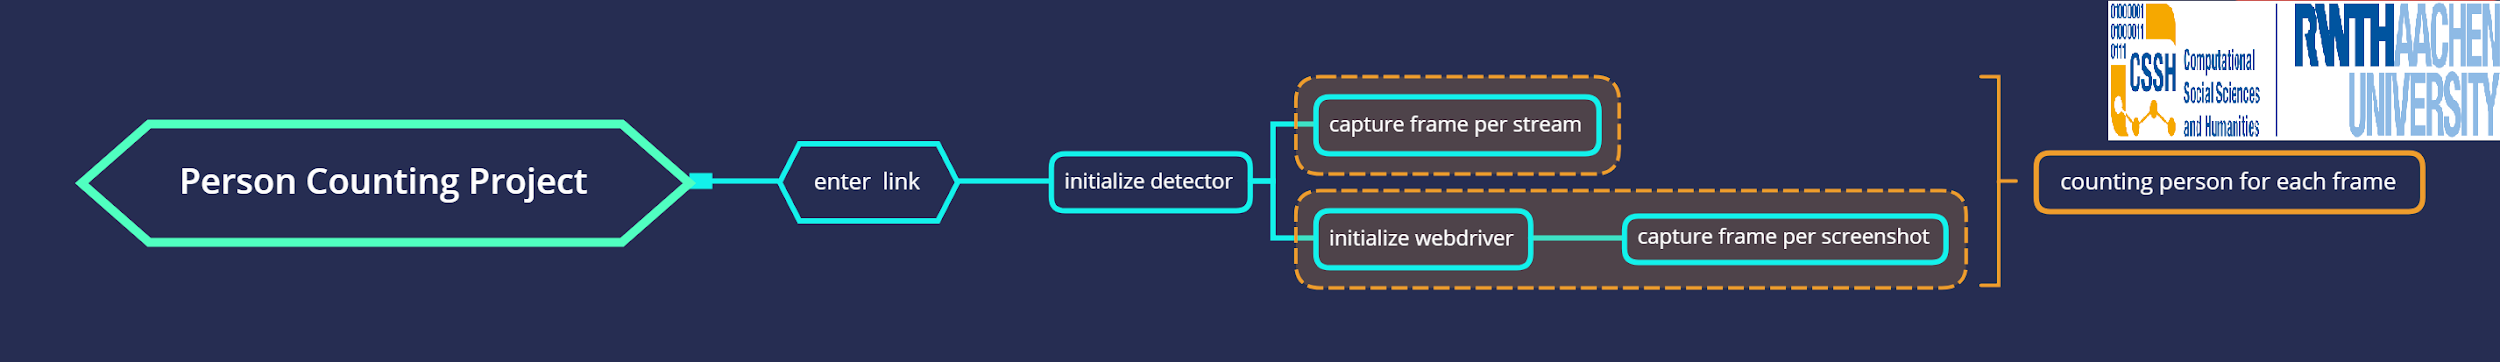
\includegraphics[width=\textwidth]{figs/pipeline.png}
\caption{Pipeline shows } \label{fig1}
\end{figure}

 Figure \ref{fig1} shows the basic pipeline of the person counting project. The first step of the pipeline is to enter the stream link of a webcam. Then the detector should be initialized. In this project, we use a detector based on Python library ImageAI. When initializing the detector, the model(retina net, yolov3, yolo tiny), detect speed could be defined. After initializing the detector, there are two different methods to capture frames. The first one is capture frame per stream, it captures the frame simply from the stream link. The Python library Streamlink has been used. Another method is capture frame per screenshot, it applies the webdriver to open browser automation and takes screenshots and stores them as frames. The final step of the pipeline is counting person for each frame by the detector we initialized before.  


\section{Problem}
During the development of this whole project we encountered a few problems that are worthy to be recorded. 

\subsection{Advertisements}
When we visit a webcam via browser, Ads are shown before we have the view of the webcam. If we take a screenshot once we open the webcam, we get an unwanted image to be analyzed, thereby, we attach a line code of sleeping about 15 seconds to make sure we skip the ads.

\subsection{Prerequisite for the way of screenshot}
To count the pedestrians via opening a browser, taking screenshots, you must have a web browser and download a third-party browser webdriver from \href{https://www.seleniumhq.org/download/}{selenium}. For webdrivers, we can pack webdrivers of top browsers to our project, but users still need to install a corresponding browser.

The browser may also need to provide the support of adobe flash, by which we are able to open a webcam by using the stream link without any problems.

\subsection{The type of input images to the detector}
For the screenshot method, there is only one input type of images to the detector, which is a real image. We take a screenshot first and then input it to the detector and detect how many pedestrians in the images. However, for the stream method, there are two possible input types. One is array, and the other is real image. The frame we captured from the stream is an array like image, therefore it can be directly inputted into the detector. Another input type is real image, we first capture the frame from the stream and use OpenCV to store it as a real image, after that input it into the detector. These two possible input types show different results. The following two figures \ref{fig2.1}, \ref{fig2.2} show the difference between these two input types. Both figures apply resnet algorithm with normal speed. But figure \ref{fig2.1}(input type: real image) performs better than figure\ref{fig2.2}(input type: array). With the first input type, the detector has detected 26 pedestrians, meanwhile with the second input type only has detected 17 pedestrians. This may due to the different RGB. (The second one has the blue background color.) 
\begin{figure}
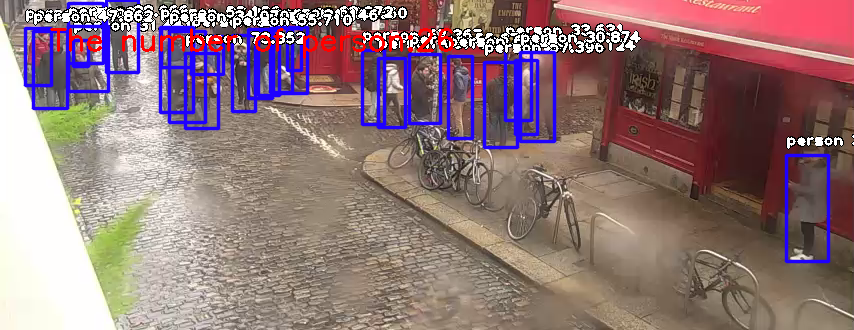
\includegraphics[width=\textwidth]{figs/problem_imgtype1.png}
\caption{Results of same image with input type real image} \label{fig2.1}
\end{figure}

\begin{figure}

	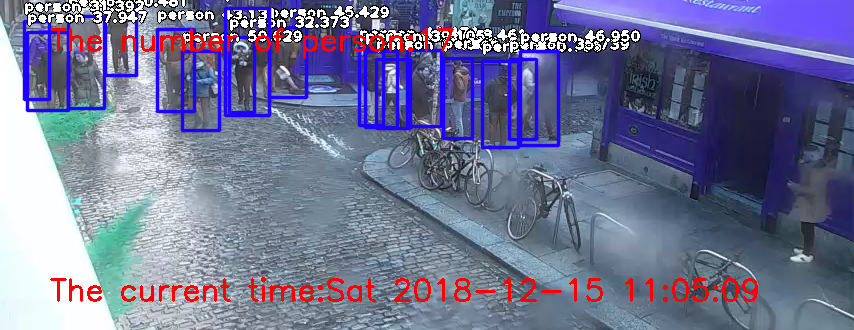
\includegraphics[width=\textwidth]{figs/problem_imgtype2.png}
	\caption{Results of same image with input type array} \label{fig2.2}
\end{figure}

\subsection{Variation of the results}
The results of method capturing frame from the stream (input type: real image) are different to the results of algorithms comparison. The following two figures show the difference. Figure \ref{fig3.1} is the result of method capturing frame from the stream (input type: real image), figure \ref{fig3.2} is the result of algorithm comparison. Both of them apply resnet model and the same baseline. However, they have different detection results. We could find that the figure \ref{fig3.2} not only detects more pedestrian but also has a higher percentage probability of detection. The reason for it is still not clear.  
\begin{figure}
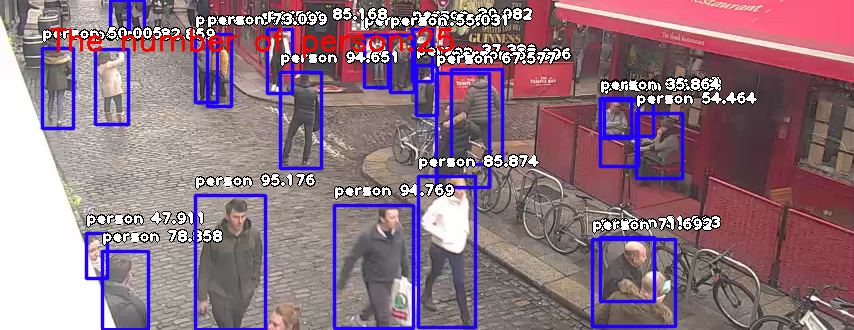
\includegraphics[width=\textwidth]{figs/problem_variant2.png}
\caption{result from the core method} \label{fig3.1}
\end{figure}

\begin{figure}
	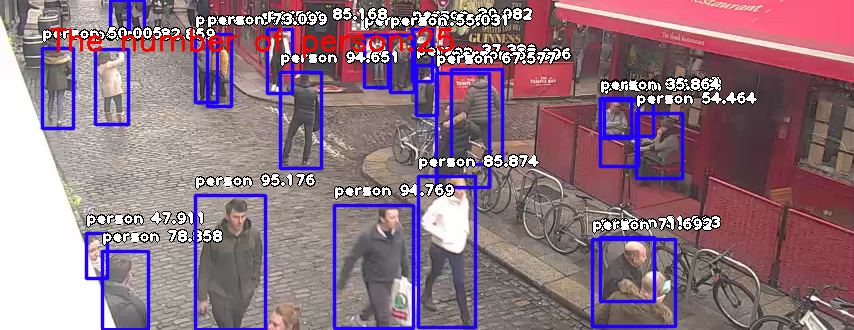
\includegraphics[width=\textwidth]{figs/problem_variant2.png}
	\caption{result during methods comparison} \label{fig3.2}
\end{figure}

\subsection{Comparison of two methods}
Although it seems method capture frame per stream is better than method capture frame per screenshot, the second method still gets some advantages in contrast to the first one.  For example, the second method can only capture frames for stream link, which means it can only capture frames from a live video but not recorded videos or uploaded videos online. Counting pedestrian with recorded videos or uploaded videos online could be handled with the screenshot method.

\section{Comparison}
This section aims at explaining how the algorithms of pedestrian detection in our project work, by which we have an overview of the idea of them. By looking into these methods, we can figure out drawbacks and advantages of them, so that we are able to understand the evaluation result in the section of evaluation without effort. Since the project is based on the python library ImageAI which integrates three modern algorithms YOLOv3, Tiny YOLOv3, and RetinaNet. All of them are trained on COCO dataset. 

Most of the traditional methods of object detection were devised to detect objects by sliding proposing template boxes at different scales from top left to bottom right of an image, for instance, the technique of sliding window. Intuitively, these techniques consume much effort on the progress of matching, since they traverse all available regions by sliding the window/template to do a match. Besides, objects probably occur in an image at any size so that the different sizes of sliding windows/templates must be given. In the following, we first introduce a new method with a different designing idea called YOLOv3. 

\subsection{YOLOv3}
YOLO is short for You Only Look Once that directly indicates that you only look once at an image to detect objects and locate where they are. YOLO is a new approach different from other modern approaches of object detection because it reframes object detection as a regression problem by means of bounding boxes and associated class probabilities. The postfix “v3” indicates the version of YOLO which implies that there are some improvements in current version v3 compared to v1 and v2, but the basic framework does not have many changes, so here we present the base idea by means of the detail of YOLOv1. The YOLO detection system is quite simple, only 3 core steps shown in ~\ref{fig4}
\begin{figure}
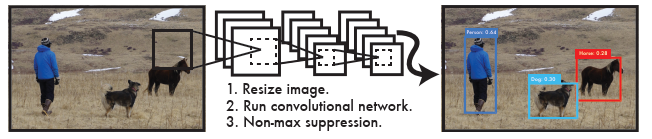
\includegraphics[width=\textwidth]{figs/YOLO_System.png}
\caption{The concise structure of YOLO detection system comprising 3 steps. Source: ~\cite{ref_yolov1}} \label{fig4}
\end{figure}

The main idea of YOLO is to divide an image into a 7x7 grid cells. For each grid cell, we predict M bounding boxes which are represented by a quintuple (x, y, w, h, con). The first two entries (x, y) point out the offset of the center of an object relative to the cell coordinate, (w, h) are the width and height of the predicted bounding boxes and con is the confidence defined as $$Pr(object) * IOU_{pred}^{truth}$$. If the center of the object falls in a cell, then $$Pr(object)$$ = 1, otherwise 0. Then we compute the Intersection Over Union (IOU) of the ground truth and the predicted bounding box, so confidence is a fractional value shows how confident an object exists in that grid cell. Besides, each grid cell predicts C conditional class probabilities $$Pr(class_i|object)$$. Note all bounding boxes of a grid cell share the one copy of the C conditional class probabilities. By means of these parameters the model looks like below in the figure. So far we can infer that the class probabilities of a bounding box is computed as: $$Pr(class_i|object) * Pr(object) * IOU_{pred}^{truth}$$.

All above is a rough description of YOLO method and we omit many details of the network and training strategies and so on. In summary, this method has the following advantages.

\begin{itemize}
	\item YOLO runs extremely fast, because the pipeline of the YOLO detection system is very simple like in the Figure. According to the evaluation result in the paper of YOLO v1 it is faster than other methods like Fast R-CNN.
	\item YOLO makes predictions by looking at the entire image instead of local regions so that it is prone to have less false positives that detect backgrounds as objects.
	\item YOLO is capable of learning generalizable representations, which means can detect different types of images even if we train the network on natural images and test it on artwork.
\end{itemize}

Of course, there are some limitations of YOLO. First, as mentioned in the beginning, YOLO tries to learn reasonable bounding boxes enclosing objects. If objects in a new or weird aspect ratio then the detection results become worse. Second, YOLO (v1) suffers from localization errors compared to other Fast R-CNN. Third, YOLOv1 gives two bounding boxes for each grid cell.
\begin{figure}
\includegraphics[width=\textwidth]{figs/YOLO_model.png}
\caption{YOLO Model. Dividing the image into an S x S grid cells and predicting B bounding boxes for each cell. Source: ~\cite{ref_yolov1}} \label{fig5}
\end{figure}
As the YOLOv1 lag behind the Fast R-CNN at mean average precision (mAP) due to the disadvantages, the better version called YOLOv2 was issued by the researchers. They came up with a few strategies to improve the mAP by decreasing localization errors. The more specific descriptions are listed in the Figure. 3, in which we can directly observe the advancement.
\begin{figure}
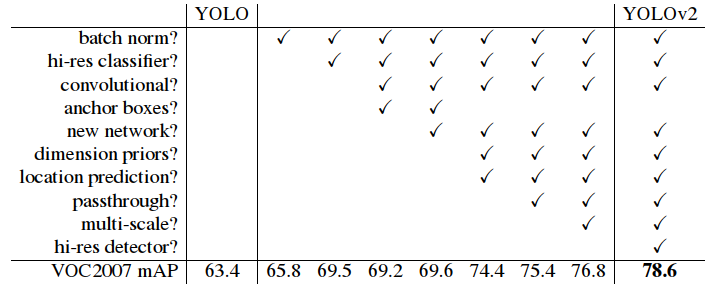
\includegraphics[width=\textwidth]{figs/YOLOv1_to_v2.png}
\caption{The advancement of YOLOv2 compared to YOLO by attaching given strategies. source: ~\cite{ref_yolov2}} \label{fig6}
\end{figure}
The mAP increases by attaching one optimization strategy at each timestep. Nevertheless, the optimization strategy of anchor boxes does not give a positive gain in mAP, but in the paper it mentions that the recall (true positives over false+true positives) in this case increases.
In the evolution progress of YOLOv2 to v3, like the authors wrote: just a bunch of small changes that make it better. The main small changes are residual network integrated and feature pyramid network (FPN) adopted. In addition, the number of convolutional layers increases at 53 compared to 19 of YOLOv2. 

\subsection{Tiny YOLOv3}
Tiny YOLOv3 is a simplified version of YOLOv3 by cutting down some convolutional layers for extracting features. As if its prefix “Tiny” implies, it is lightweight, namely a tradeoff between runtime and precision. It could run faster than YOLOv3, but the precision would be a bit worse. 

\subsection{RetinaNet}
The detectors which have the highest accuracy of object detection are two-stage detectors. The YOLO detector is a one-stage detector. Roughly speaking, the difference between two-stage and one-stage detectors is that the pipeline of two-stage detectors is more complicated, as the two-stage detectors invest much labor in extracting a sparse set of proposal regions at different scales, aspect ratios and locations in the first stage, by which classifies less number of regions in the second stage. The YOLO detector made a tradeoff between accuracy and speed. Although its performance is not one of the best, it is able to detect objects in real time in the case of ensuring a decent accuracy. However, the YOLO detector is unlikely to increase the accuracy even with a larger compute budget. In contrast, the goal of RetinaNet is to look up if the one-stage detector is able to outperform the accuracy of two-stage detectors when running at similar or faster speed. Obviously, RetinaNet is a one-stage detector, which is named for densely sampling of object locations in an input image. 

In order to achieve that goal, RentinaNet introduces a novel loss function named as Focal Loss by adding two factors to standard cross entropy loss. The reason for the modification of loss function is that the problem of the large class imbalance occurs very often in classification tasks. The class imbalance is likely to overwhelm the cross-entropy loss for minimizing the loss during the training of an object detector, since the detector tends to stand on the side of the majorities that dominates the loss. In particular, we are often unable to collect positive training examples as many as negative training examples. On the contrary, in many situations the amount of positive examples is much less than the amount of negative examples, which leads to class imbalance especially if there is a dense detector. Obviously, if the proportion of positives and negatives is 1:99 and the standard cross entropy loss for binary classification is given as in the Equation $$CE(p,y) = -log(p) if y =1, otherwise -log(1-p)$$ where $$y \in {+1, -1}$$ indicates ground-truth class and $$p \in [0,1]$$ is the probability of predicting the class with label y = 1, to reduce the error the detector can simply predict all input examples as negative (non-object) then achieving the accuracy of 99\% result in an amazing perfect detector. Nevertheless, that detector is quite poor. The problem was that we treat all examples equally, even if they are not. RetinaNet proposes to modify the loss function in two steps.

\begin{itemize}
	\item Attach a weighting factor $\alpha \in [0,1]$, for positive class and $1 - \alpha$ for negative class. In practice $\alpha$ might be configured by inverse class frequency, similar as inverse document frequency of TF-IDF. The more the class labels occur, the less the weighting factor is.
	\item Although $\alpha$ balances the importance of positive and negative examples, it does not take the easy and hard examples into account. Intuitively, the harder an example to be classified, the more important the example is. According to this idea, RetinaNet attached a modulating factor $(1-p_t)^\gamma$ to the cross-entropy loss where $\gamma \geq 0$ and $p_t = p$ if y = 1, otherwise $1-p$. What’s more, the focal loss is visualized with different values of $\gamma$ in the ~\ref{fig7}.
\end{itemize}

\begin{figure}
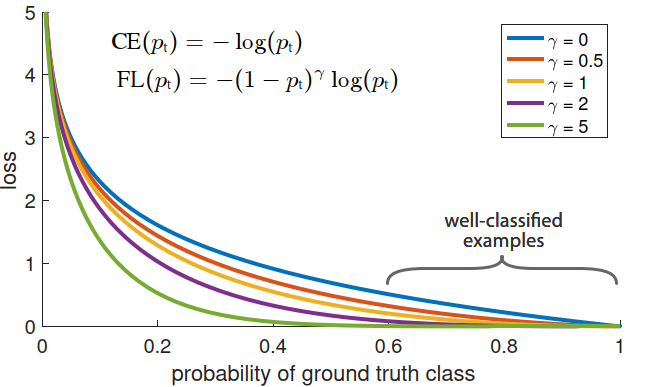
\includegraphics[width=\textwidth]{figs/loss_with_gammas.png}
\caption{$\gamma = 0$ implies the standard cross entropy loss which is represented by the blue curve. With positive $\gamma$ the focal loss is reduced. The green curve with the highest $\gamma$ value shows that the focal loss is reduced relatively large for hard examples ($p_t \leq 0.4$). source: ~\cite{ref_retinanet}} \label{fig7}
\end{figure}

So far we present how RetinaNet solves the problem of class imbalance by means of a novel focal loss function. Equally important part is that RetinaNet detector has a simple and clear pipeline of its networks. It comprises a backbone network and two task-specific subnetworks. The backbone network takes efforts to compute a convolutional feature map over an entire image. The backbone’s output, namely a convolutional feature map, is fed into the first task-specific subnetwork which is responsible for performing convolutional object classification. The second subnetwork performs convolutional bounding box regression. It is visualized in the ~\ref{fig8}.

\begin{figure}[H]
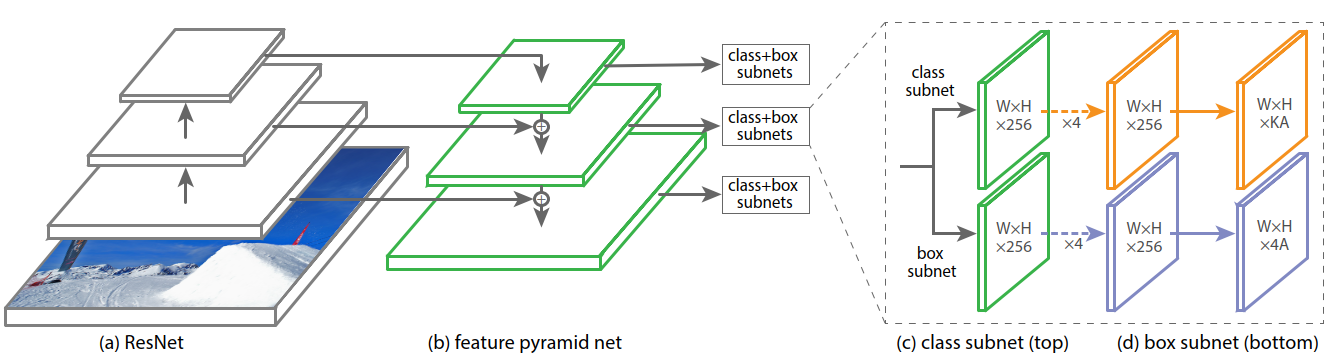
\includegraphics[width=\textwidth]{figs/RetinaNet_network.png}
\caption{(a) and (b): Backbone network is a Feature Pyramid Network (FPN) built on top of the ResNet (Residual Network) architecture. Go through the pathway of ResNet bottom-up to downscale getting feature maps at different scales. Applying skip connections (Residual) binds ResNet and FPN at each scale so that the FPN is able to upsample smoothly without losing more details. (c) and (d): subnetworks of classification on backbone’s outputs and bounding box regression. source: ~\cite{ref_retinanet}} \label{fig8}
\end{figure}

In summary, the performance of RetinaNet can be proved by the experiment result in the ~\ref{fig9}.
\begin{figure}[htbp]
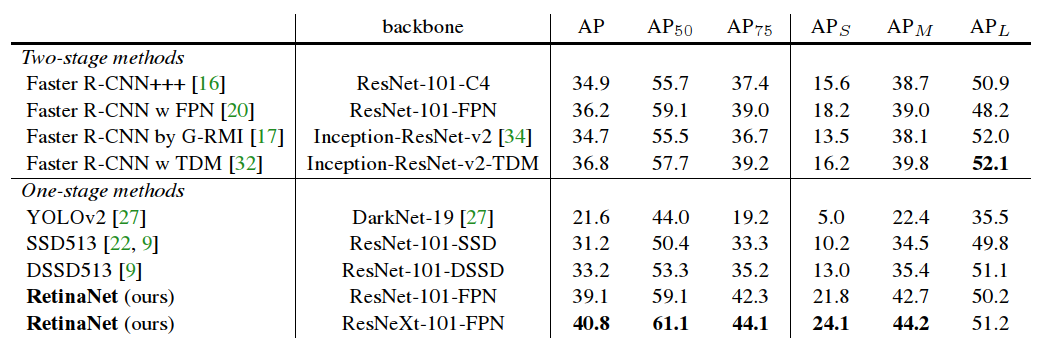
\includegraphics[width=\textwidth]{figs/RetinaNet_object_detection.png}
\caption{Evaluated on COCO test-dev. RetinaNet achieves top results and outperforms one-stage and two-stage detectors. Source: ~\cite{ref_retinanet}} \label{fig9}
\end{figure}


\section{Evaluation}
From the previous chapter, we go through the detail of three methods/algorithms that are applied in our project. In this chapter, the evaluation strategies and hypotheses and the result will be represented. We do not present the part of training as the three models pre-trained. 

\subsection{Test Dataset}
All datasets and CSV files could be found in \url{https://drive.google.com/open?id=1ELg5LJoU0coNjNZdjSXeaZLv6cI_jnKP}.

The detection results are stored in folder \textit{\textbf{dublin\_day}} 
and \textit{\textbf{dublin\_night}}. The baseline images are stored in folder \textit{\textbf{dublin\_day\_baseline}} and \textit{\textbf{dublin\_night\_baseline}}. The results of algorithms comparison are stored in folder \textit{\textbf{algos\_dublin\_day}} and \textit{\textbf{algos\_dublin\_night}}. There is a CSV folder store all results of CSV files. The results of detection are stored in \textit{\textbf{dublin\_day.csv}} and \textit{\textbf{dublin\_night.csv}}. Labeled results are stored in \textit{\textbf{labeled\_dublin\_day.csv}} and \textit{\textbf{labeled\_dublin\_night.csv}}. The scores results included day and night are stored in \textit{\textbf{dublin\_scores.csv}}. For the algorithms comparison, there are two CSVs, namely \textit{\textbf{Algos\_dublin\_day.csv}} and \textit{\textbf{Algos\_dublin\_night.csv}}, show the detection results of three algorithms (resnet, yolov3, yolo\_tiny) from randomly select 15 images of the \textit{\textbf{dublin\_day}} and \textit{\textbf{dublin\_night}} dataset. And six CSVs for the labeled results of three algorithms and day and night. The scores result included day and night of three algorithms are stored in \textit{\textbf{algo\_dublin\_scores.csv}}
\\

Intuitively, in the test phase the model can be tested on real data, so the test dataset is constructed by taking images from an online webcam and includes 100 images. We executed our python program to collect 50 images from a webcam of a walking street in Dublin in the daytime and nighttime separately. The webcam took images periodically, namely at every 3 minutes, to ensure an image distinguished from its neighbor images, because of people on that street flow by the webcam. After collecting these 100 images, we counted pedestrians in each image by ourselves and store the number in a CSV file. In order to count the number of pedestrians precisely, we also store the baseline datasets. Note that the counted number is inexact but approximately, since the scene of an image often contains many people who are very close to each other, resulting in occlusion. In addition, pedestrians were far from the webcam so that it was hard to recognize them that occurred in an image with a very small size. Thereby, we crop images and took the bottom half part of each image to ensure the test results are not in a quite tough situation. The following two figures \ref{fig10.1}, \ref{fig10.2} show the conditions before cropped and after cropped. So the pedestrians in the alley could not be considered. 

\begin{figure}[H]
	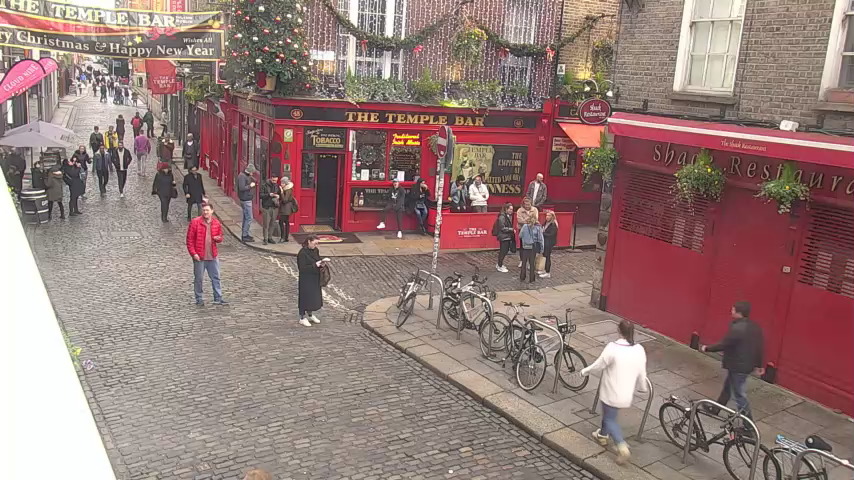
\includegraphics[width=\textwidth]{figs/eva_original_img.png}
	\caption{original image} \label{fig10.1}
\end{figure}
\begin{figure}
	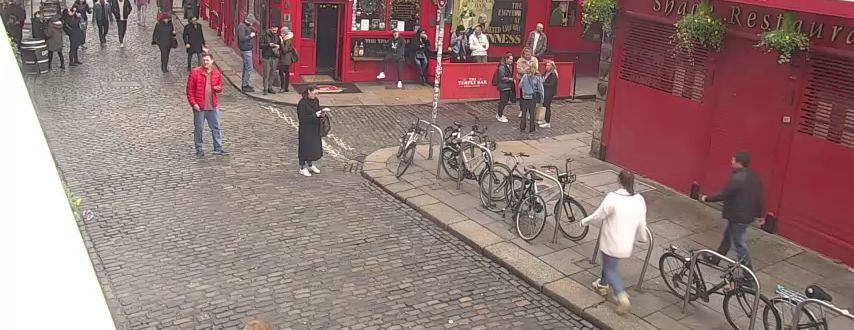
\includegraphics[width=\textwidth]{figs/eva_cropped_img.png}
	\caption{cropped image} \label{fig10.2}
\end{figure}


What is more, because of the counted number of images is inexact, it is necessary to make some subsidiary labels. For instance, make some label like 0-0.2 quantile, 0.2 quantile - 0.4 quantile, etc. and if the counted number is greater than the median and the difference between the detected number and the counted number is smaller than the standard deviation of the greater part, we assume they are the same, if the counted number is smaller than median and the difference between the detected number and the counted number is smaller than the standard deviation of the smaller part, we assume they are the same. We use these subsidiary labels to evaluate the dataset. 


\subsection{Strategies and Hypotheses}
In order to evaluate these three pre-trained models properly, we make a few reasonable strategies. We randomly select 15 images from each baseline dataset(day and night) and apply them in three different algorithms, after that we use the same method to evaluate it.

\paragraph{\textbf{Daytime and Nighttime}} In practice, the illumination in the daytime and in the nighttime has a huge difference and the change of illumination will influence the accuracy of object detection, even if the human is unable to have a good performance in the nighttime, especially the environment is very dark. We let each model perform on the dataset of daytime and the dataset of nighttime alternatively.  Roughly speaking, we hypothesize that the test accuracy on the dataset of nighttime is unlikely to be as good as the accuracy on the dataset of daytime for each model.\\



The following table \ref{tab1} and table \ref{tab2} show the result of the detected number, time and the counted number in dataset day and night. From these two tables, we could find that the accuracy is not very high. Because of the counted number of images is inexact, it is necessary to make some subsidiary labels.\\

The following table \ref{tab3} and table \ref{tab4} show the result of the labeled dataset in day and night. We add three subsidiary labels to help for the evaluation. label\_detected and label\_counted show the range of the detected number and counted number. From 0 - 0.2 quantile, 0.2 quantile - 0.4 quantile, etc. and if the counted number is greater than the median and the difference between the detected number and the counted number is smaller than the standard deviation of the greater part, we assume they are the same, if the counted number is smaller than median and the difference between the detected number and the counted number is smaller than the standard deviation of the smaller part, we assume they are the same.  


\begin{table}[H]
	\csvautotabular[respect underscore=true, 
	%filter={\value{csvrow}<5}
	]{csvs/Dublin_day.csv}\\
	\caption{result of dublin day}
	\label{tab1}
\end{table}
\begin{table}[H]
	\csvautotabular[respect underscore=true,
	%filter={\value{csvrow}<5}
	]{csvs/Dublin_night.csv}\\
	\caption{result of dublin night}
	\label{tab2}
\end{table}

\begin{table}[H]
	\centering
	\resizebox{\textwidth}{!}{
		\begin{tabular}{l c r}
			\csvautotabular[respect underscore=true,
			%filter={\value{csvrow}<5}
			]{csvs/labeled_dublin_day.csv}
			
	    \end{tabular}}
\caption{labeled result of dublin day}
\label{tab3}
\end{table}

\begin{table}[H]
	\centering
	\resizebox{\textwidth}{!}{
		\begin{tabular}{l c r}
			\csvautotabular[respect underscore=true,
			%filter={\value{csvrow}<5}
			]{csvs/labeled_dublin_day.csv}
			
	\end{tabular}}
	\caption{labeled result of dublin day}
	\label{tab4}
\end{table}

\begin{table}[H]
	\centering
	\resizebox{\textwidth}{!}{
		\begin{tabular}{l c r}
			\csvautotabular[respect underscore=true,
			%filter={\value{csvrow}<5}
			]{csvs/labeled_dublin_night.csv}
			
	\end{tabular}}
	\caption{labeled result of dublin night}
	\label{tab5}
\end{table}

\begin{table}[H]
	\centering
	\resizebox{\textwidth}{!}{
		\begin{tabular}{l c r}
			\csvautotabular[respect underscore=true,
			%filter={\value{csvrow}<5}
			]{csvs/dublin_scores.csv}
			
	\end{tabular}}
	\caption{scores result of dublin}
	\label{tab6}
\end{table}



After making these subsidiary labels. We could evaluate the dataset day and night. The table \ref{tab6} shows the accuracy, f1 score, precision score, r2 score, the accuracy with a label, f1 with a label, precision with a label, recall with label and accuracy with bool. From this table, we could find that the accuracy with range of night is 52\% and of the day is 58\%. However, when it applies accuracy with bool, the accuracy of night stays but the accuracy of the day increases to 72\%. In short, the detector performs better in the daytime.

\paragraph{\textbf{Evaluation of algorithms}}  We randomly select 15 images from each baseline dataset (day and night) and apply them in three different algorithms, after that we use the same method to evaluate it. 

\begin{sidewaystable}[h]
	\flushright
	\sisetup{round-mode=places, round-precision=3}
	\resizebox{\textwidth}{13mm}{
		\begin{tabular}{ccSSSSSSSSSS}
			\csvautotabular[respect underscore=true
			%filter={\value{csvrow}<5}
			]{csvs/algos_dublin_scores.csv}
			
	\end{tabular}}
	\caption{scores result of three algorithms dublin}
	\label{tab7}
\end{sidewaystable}

This table \ref{tab7} shows the scores of three different algorithms in day and night. In the night time, the accuracy with range of algorithm resnet, yolov3 and yolo\_tiny are 47\%, 27\%, and 40\%. And the accuracy with bool of them is 60\%, 20\%, and 6.7\%. Obviously, resnet is the best algorithm in the night. What is more, yolo\_tiny performs better than yolov3 in the night when we evaluate with range, and yolov3 performs better than yolo\_tiny in the night when we evaluate with bool.  In the daytime, the accuracy with range of algorithm resnet, yolov3 and yolo\_tiny are 100\%, 93\%, and 73\%. And the accuracy with bool of them is 67\%, 60\%, and 33\%. Resnet is the best algorithm in the daytime without doubt regarding these two scores. Meanwhile, yolov3 performs better than yolo\_tiny in the daytime.

In short, resnet is the best algorithm no matter it is daytime or night time. 





% \begin{table}
% \caption{Table captions should be placed above the
% tables.}\label{tab1}
% \begin{tabular}{|l|l|l|}
% \hline
% Heading level &  Example & Font size and style\\
% \hline
% Title (centered) &  {\Large\bfseries Lecture Notes} & 14 point, bold\\
% 1st-level heading &  {\large\bfseries 1 Introduction} & 12 point, bold\\
% 2nd-level heading & {\bfseries 2.1 Printing Area} & 10 point, bold\\
% 3rd-level heading & {\bfseries Run-in Heading in Bold.} Text follows & 10 point, bold\\
% 4th-level heading & {\itshape Lowest Level Heading.} Text follows & 10 point, italic\\
% \hline
% \end{tabular}
% \end{table}


% \noindent Displayed equations are centered and set on a separate
% line.
% \begin{equation}
% x + y = z
% \end{equation}
% Please try to avoid rasterized images for line-art diagrams and
% schemas. Whenever possible, use vector graphics instead (see
% Fig.~\ref{fig1}).

% \begin{figure}
% \includegraphics[width=\textwidth]{fig1.eps}
% \caption{A figure caption is always placed below the illustration.
% Please note that short captions are centered, while long ones are
% justified by the macro package automatically.} \label{fig1}
% \end{figure}

% \begin{theorem}
% This is a sample theorem. The run-in heading is set in bold, while
% the following text appears in italics. Definitions, lemmas,
% propositions, and corollaries are styled the same way.
% \end{theorem}
% %
% % the environments 'definition', 'lemma', 'proposition', 'corollary',
% % 'remark', and 'example' are defined in the LLNCS documentclass as well.
% %
% \begin{proof}
% Proofs, examples, and remarks have the initial word in italics,
% while the following text appears in normal font.
% \end{proof}
% For citations of references, we prefer the use of square brackets
% and consecutive numbers. Citations using labels or the author/year
% convention are also acceptable. The following bibliography provides
% a sample reference list with entries for journal
% articles~\cite{ref_article1}, an LNCS chapter~\cite{ref_lncs1}, a
% book~\cite{ref_book1}, proceedings without editors~\cite{ref_proc1},
% and a homepage~\cite{ref_url1}. Multiple citations are grouped
% \cite{ref_article1,ref_lncs1,ref_book1},
% \cite{ref_article1,ref_book1,ref_proc1,ref_url1}.
%

% ---- Bibliography ----
%
% BibTeX users should specify bibliography style 'splncs04'.
% References will then be sorted and formatted in the correct style.
%
\bibliographystyle{splncs04}
\bibliography{mybibliography}

\begin{thebibliography}{8}
\bibitem{ref_yolov1}
Author, Joseph Redmon and Santosh Kumar Divvala and Ross B. Girshick and Ali Farhadi: You Only Look Once: Unified, Real-Time Object Detection. Journal \textbf{CoRR}, (2015)

\bibitem{ref_yolov2}
Author, Joseph Redmon and Ali Farhadi: YOLO9000 Better, Faster, Stronger, Journal \textbf{CoRR}, (2016)

\bibitem{ref_yolov3}
Author, Joseph Redmon and Ali Farhadi: YOLOv3: An Incremental Improvement, Journal \textbf{CoRR}, (2018)

\bibitem{ref_retinanet}
Author, Tsung-Yi Lin and Priya Goyal and Ross B. Girshick and Kaiming He and Piotr D.: Focal Loss for Dense Object Detection, Journal \textbf{CoRR}, (2017)

\bibitem{ref_imageai}
ImageAI Github Homepage, \url{https://github.com/OlafenwaMoses/ImageAI}. Last accessed 04.01.2019


% \bibitem{ref_article1}
% Author, F.: Article title. Journal \textbf{2}(5), 99--110 (2016)

% \bibitem{ref_lncs1}
% Author, F., Author, S.: Title of a proceedings paper. In: Editor,
% F., Editor, S. (eds.) CONFERENCE 2016, LNCS, vol. 9999, pp. 1--13.
% Springer, Heidelberg (2016). \doi{10.10007/1234567890}

% \bibitem{ref_book1}
% Author, F., Author, S., Author, T.: Book title. 2nd edn. Publisher,
% Location (1999)

% \bibitem{ref_proc1}
% Author, A.-B.: Contribution title. In: 9th International Proceedings
% on Proceedings, pp. 1--2. Publisher, Location (2010)

% \bibitem{ref_url1}
% LNCS Homepage, \url{http://www.springer.com/lncs}. Last accessed 4
% Oct 2017
\end{thebibliography}
\end{document}
